\documentclass[tikz,border=8pt]{standalone}
% Shared look for every TikZ diagram. Load with % Shared look for every TikZ diagram. Load with % Shared look for every TikZ diagram. Load with \input{../../tools/tikz-style.tex}
\usepackage[T1]{fontenc}
\usepackage{lmodern}
\renewcommand{\sfdefault}{lmr}  % diagrams use the same serif as the text
\usetikzlibrary{arrows.meta, positioning, shapes.geometric, calc, fit, backgrounds}
\definecolor{cblue}{HTML}{4C78A8}
\definecolor{corange}{HTML}{F58518}
\definecolor{cgreen}{HTML}{54A24B}
\definecolor{cred}{HTML}{E45756}
\definecolor{cpurple}{HTML}{B279A2}
\definecolor{cgrey}{HTML}{6B6B6B}
\tikzset{
  every picture/.style={font=\sffamily, line width=1.2pt},
  box/.style={draw=#1, fill=#1!12, rounded corners=4pt, align=center, inner sep=7pt, minimum height=1.1cm},
  box/.default=cgrey,
  arrow/.style={-{Stealth[length=3mm]}, draw=cgrey, line width=1.4pt},
  title/.style={font=\sffamily\bfseries\Large},
  note/.style={font=\sffamily\small, text=cgrey, align=center},
}
\AtBeginDocument{\hyphenpenalty=10000 \exhyphenpenalty=10000}

\usepackage[T1]{fontenc}
\usepackage{lmodern}
\renewcommand{\sfdefault}{lmr}  % diagrams use the same serif as the text
\usetikzlibrary{arrows.meta, positioning, shapes.geometric, calc, fit, backgrounds}
\definecolor{cblue}{HTML}{4C78A8}
\definecolor{corange}{HTML}{F58518}
\definecolor{cgreen}{HTML}{54A24B}
\definecolor{cred}{HTML}{E45756}
\definecolor{cpurple}{HTML}{B279A2}
\definecolor{cgrey}{HTML}{6B6B6B}
\tikzset{
  every picture/.style={font=\sffamily, line width=1.2pt},
  box/.style={draw=#1, fill=#1!12, rounded corners=4pt, align=center, inner sep=7pt, minimum height=1.1cm},
  box/.default=cgrey,
  arrow/.style={-{Stealth[length=3mm]}, draw=cgrey, line width=1.4pt},
  title/.style={font=\sffamily\bfseries\Large},
  note/.style={font=\sffamily\small, text=cgrey, align=center},
}
\AtBeginDocument{\hyphenpenalty=10000 \exhyphenpenalty=10000}

\usepackage[T1]{fontenc}
\usepackage{lmodern}
\renewcommand{\sfdefault}{lmr}  % diagrams use the same serif as the text
\usetikzlibrary{arrows.meta, positioning, shapes.geometric, calc, fit, backgrounds}
\definecolor{cblue}{HTML}{4C78A8}
\definecolor{corange}{HTML}{F58518}
\definecolor{cgreen}{HTML}{54A24B}
\definecolor{cred}{HTML}{E45756}
\definecolor{cpurple}{HTML}{B279A2}
\definecolor{cgrey}{HTML}{6B6B6B}
\tikzset{
  every picture/.style={font=\sffamily, line width=1.2pt},
  box/.style={draw=#1, fill=#1!12, rounded corners=4pt, align=center, inner sep=7pt, minimum height=1.1cm},
  box/.default=cgrey,
  arrow/.style={-{Stealth[length=3mm]}, draw=cgrey, line width=1.4pt},
  title/.style={font=\sffamily\bfseries\Large},
  note/.style={font=\sffamily\small, text=cgrey, align=center},
}
\AtBeginDocument{\hyphenpenalty=10000 \exhyphenpenalty=10000}

\begin{document}
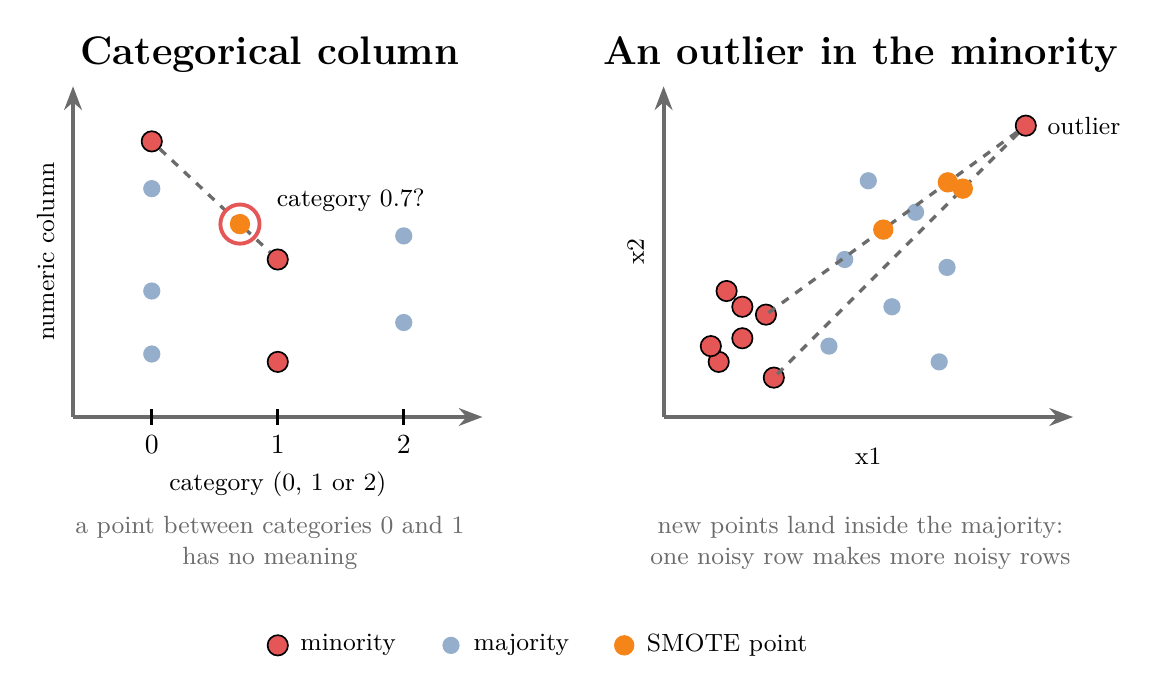
\begin{tikzpicture}[mn/.style={circle, fill=cred, draw=black, line width=0.6pt, inner sep=2.6pt},
  mj/.style={circle, fill=cblue!60, inner sep=2.2pt}, syn/.style={circle, fill=corange, inner sep=2.6pt},
  bad/.style={circle, draw=cred, line width=1.4pt, inner sep=5pt}]
  % left: a categorical column
  \begin{scope}
    \node[title] at (2.5,4.6) {Categorical column};
    \draw[arrow] (0,0) -- (5.2,0) ;
    \draw[arrow] (0,0) -- (0,4.2) ;
    \node[font=\sffamily\small] at (2.6,-0.85) {category (0, 1 or 2)};
    \node[font=\sffamily\small, rotate=90] at (-0.35,2.1) {numeric column};
    \foreach \c [count=\i from 0] in {0,1,2} {\draw (1+1.6*\i,0.1) -- (1+1.6*\i,-0.1) node[below] {\c};}
    \foreach \y in {0.8,1.6,2.9} \node[mj] at (1,\y) {};
    \foreach \y in {1.2,2.3} \node[mj] at (4.2,\y) {};
    \node[mn] (a) at (1,3.5) {}; \node[mn] (b) at (2.6,2.0) {}; \node[mn] at (2.6,0.7) {};
    \draw[cgrey, dashed] (a) -- (b);
    \node[syn] (n) at (2.12,2.45) {};
    \node[bad] at (n) {};
    \node[anchor=west, font=\sffamily\small] at (2.45,2.75) {category 0.7?};
    \node[note] at (2.5,-1.6) {a point between categories 0 and 1\\has no meaning};
  \end{scope}
  % right: an outlier in the minority class
  \begin{scope}[xshift=7.5cm]
    \node[title] at (2.5,4.6) {An outlier in the minority};
    \draw[arrow] (0,0) -- (5.2,0) ;
    \draw[arrow] (0,0) -- (0,4.2) ;
    \foreach \x/\y in {0.7,1.0/1.4,0.6/0.9,1.3/1.3,1.4/0.5,0.8/1.6,1.0} \node[mn] at (\x,\y) {};
    \foreach \x/\y in {2.3/2.0,2.9/1.4,3.2/2.6,2.6/3.0,3.6/1.9,2.1/0.9,3.5/0.7} \node[mj] at (\x,\y) {};
    \node[mn] (o) at (4.6,3.7) {};
    \node[font=\sffamily\small] at (2.6,-0.5) {x1};
    \node[font=\sffamily\small, rotate=90] at (-0.35,2.1) {x2};
    \node[anchor=west, font=\sffamily\small] at (o.east) {outlier};
    \draw[cgrey, dashed] (o) -- (1.3,1.3); \draw[cgrey, dashed] (o) -- (1.4,0.5);
    \node[syn] at (3.61,2.98) {}; \node[syn] at (2.79,2.38) {}; \node[syn] at (3.8,2.9) {};
    \node[note] at (2.5,-1.6) {new points land inside the majority:\\one noisy row makes more noisy rows};
  \end{scope}
  \node[mn] at (2.6,-2.9) {}; \node[anchor=west, font=\sffamily\small] at (2.75,-2.9) {minority};
  \node[mj] at (4.8,-2.9) {}; \node[anchor=west, font=\sffamily\small] at (4.95,-2.9) {majority};
  \node[syn] at (7.0,-2.9) {}; \node[anchor=west, font=\sffamily\small] at (7.15,-2.9) {SMOTE point};
\end{tikzpicture}
\end{document}
